\chapter{Evaluation and Results}

\section{RAG Chatbot}
The primary goal of developing the Study Buddy RAG chatbot was to gain hands-on experience with large language models (LLMs) and their application in real-world language processing tasks. %The evaluation metrics used to assess the chatbot focused on its internal performance and functionality rather than user testing:

% \begin{itemize}
%     \item \textbf{Functionality:} Ensures that all components (retriever, generator, and PDF uploader) work seamlessly together.
%     \item \textbf{Response Time:} Assesses the time taken by the chatbot to generate responses, ensuring quick and efficient interaction.
% \end{itemize}
The evaluation of the Study Buddy chatbot involved querying the chatbot both before and after inserting relevant documents. The aim was to observe how the inclusion of additional context impacts the chatbot's performance in terms of accuracy, relevance, and response quality. This internal testing was done to verify that the chatbot was ready for potential future testing by users.

\subsection{Functionality Testing}
The functionality of the chatbot was tested by ensuring that all components (retriever, generator, and PDF uploader) worked seamlessly together. This involved verifying the following:

\begin{itemize}
    \item \textbf{PDF Uploader:} Successfully uploading PDF documents and storing them in the Astra DB Vector Store.
    \item \textbf{Retriever Component:} Accurately retrieving relevant documents based on user queries.
    \item \textbf{Generator Component:} Generating coherent and contextually relevant responses using the GPT-4 model.
    \item \textbf{Integration:} Ensuring that the retriever and generator components integrate smoothly to provide comprehensive responses.
\end{itemize}

\subsection{Case Study: Impact of Document Insertion on Response Quality}
A series of specific queries were made to the Study Buddy chatbot before and after inserting a set of relevant documents. The goal was to observe changes in the quality of responses. The queries were related to complex topics that required detailed and specific information.

\textbf{Example Query 1:}
The first query was related to the topic of "orthogonal matrices" and involved asking the chatbot to explain the properties of orthogonal matrices.
\begin{itemize}
    \item \textbf{Before Document Insertion:} The chatbot provided a general and correct overview of the topic.
    \begin{figure}[H]
        \centering
        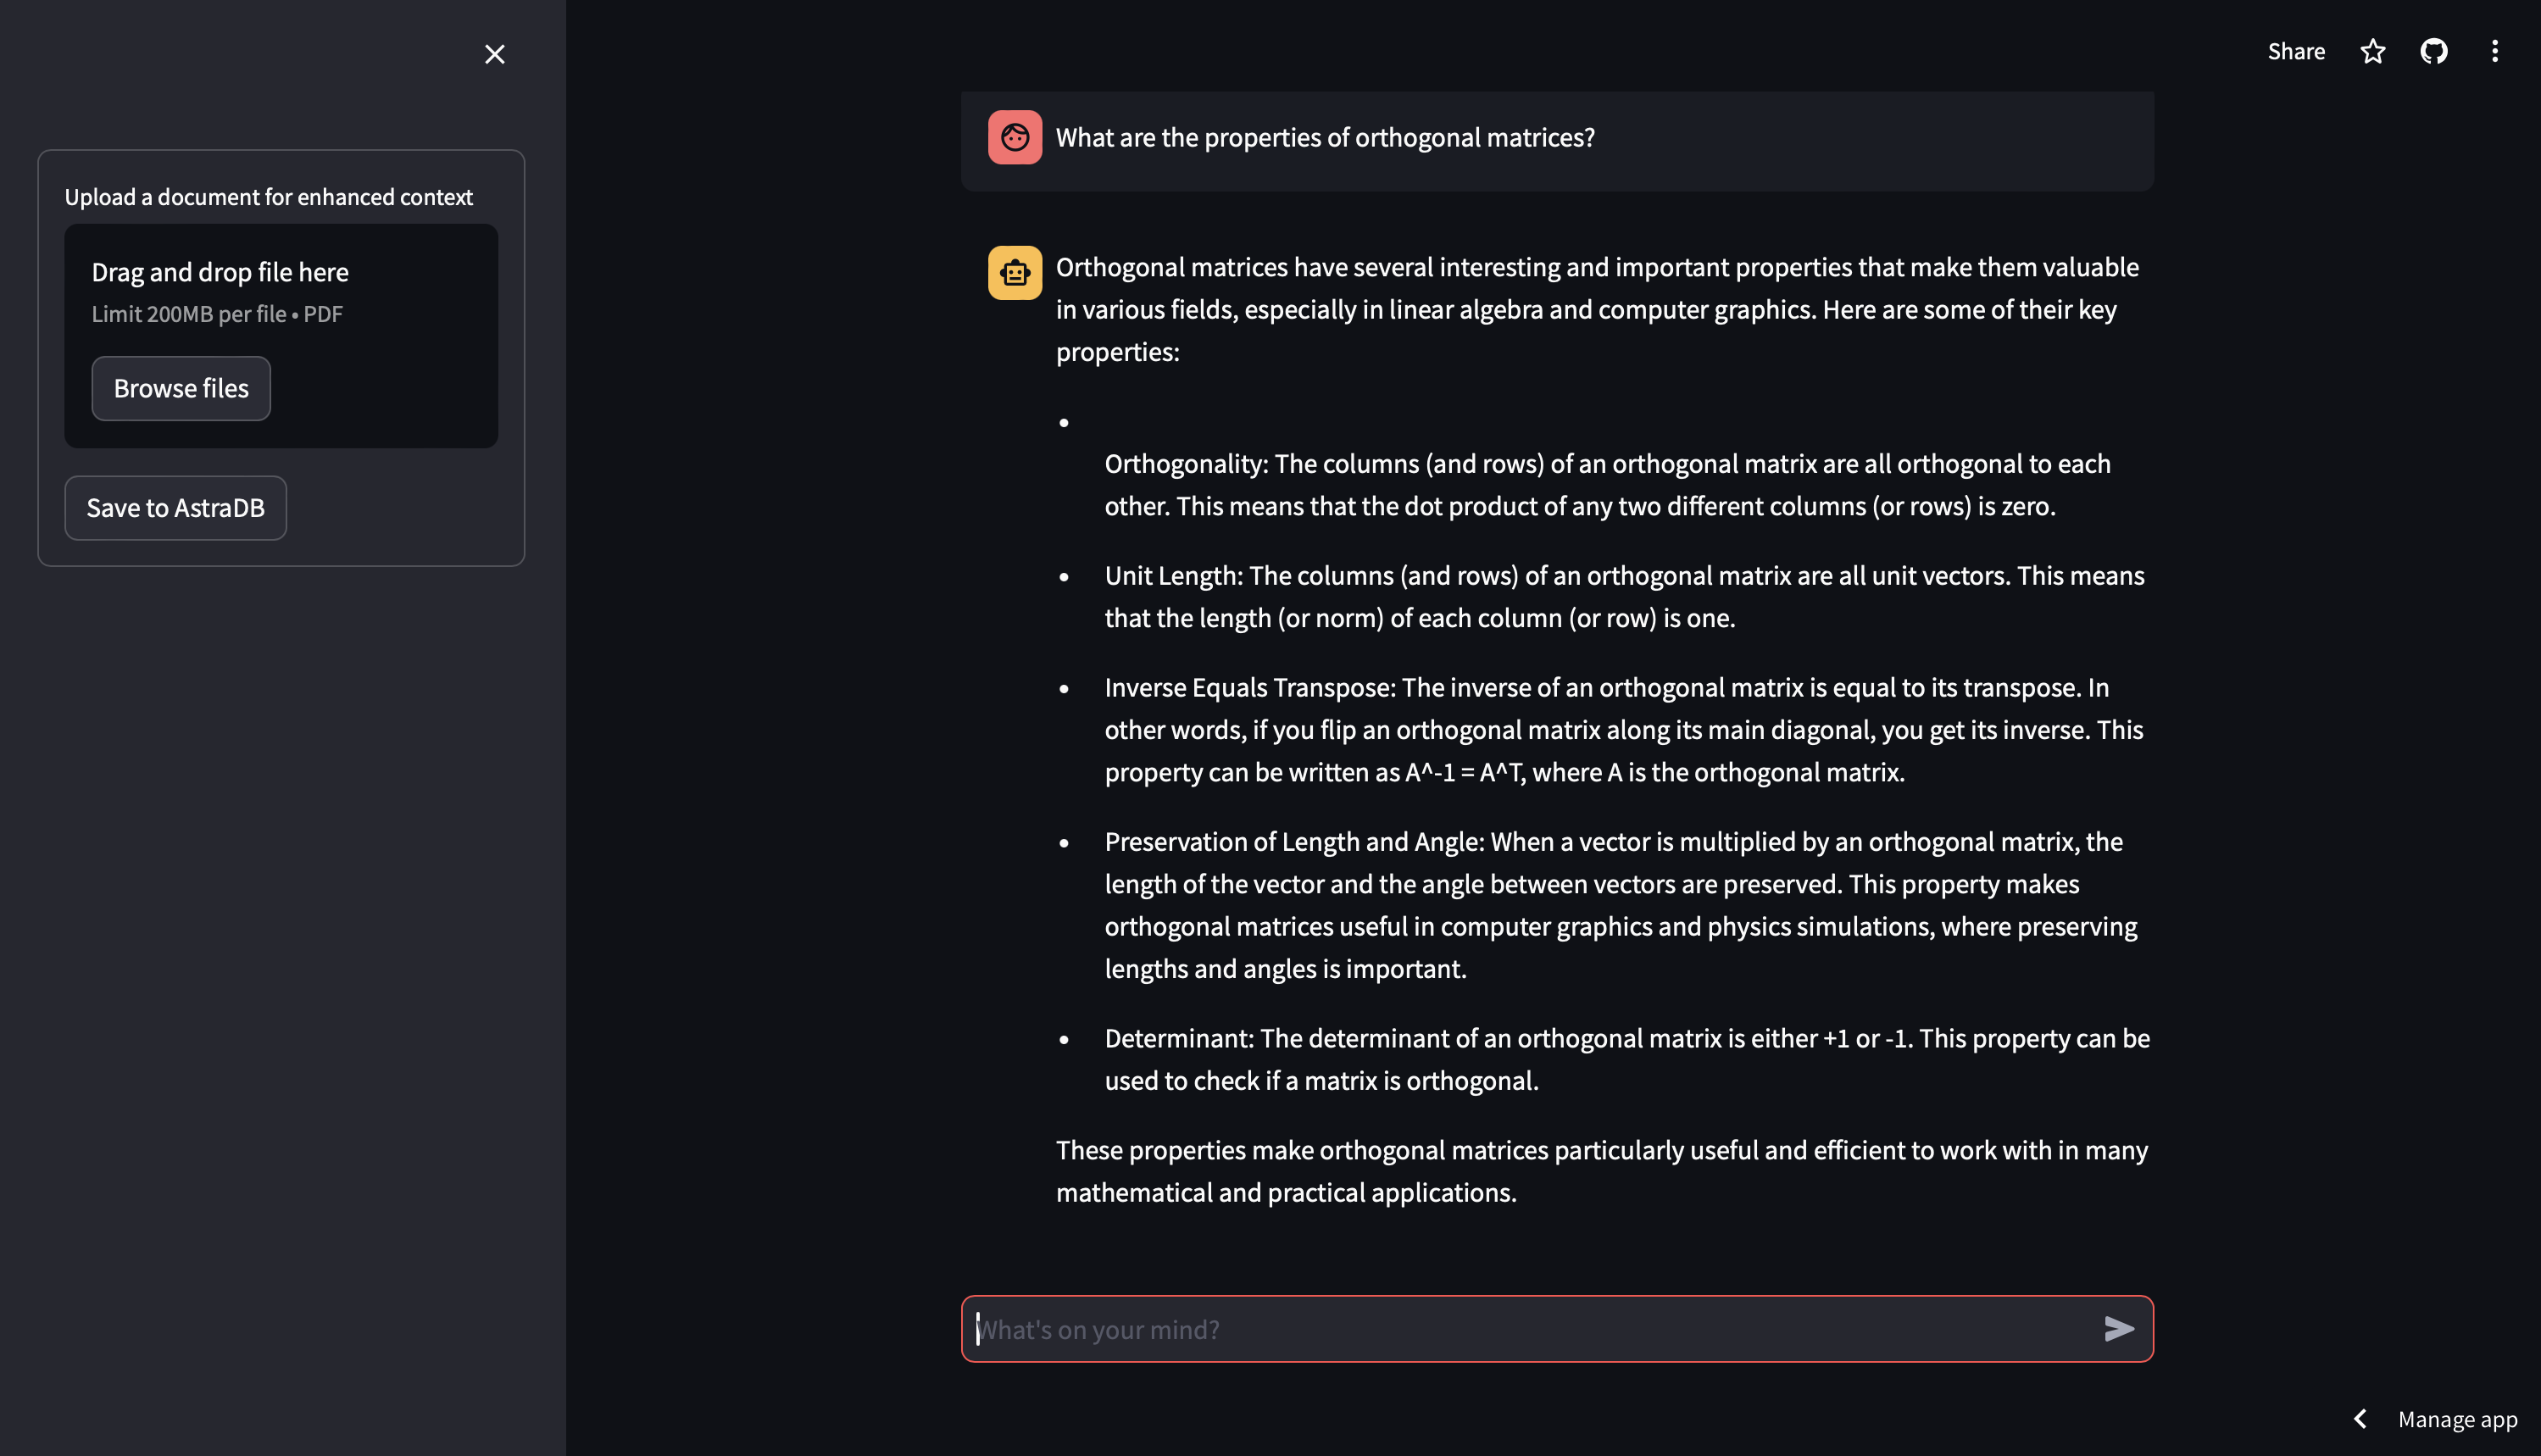
\includegraphics[width=0.8\textwidth]{figs/BeforeOrthogonal.png}
        \caption{Response before insertion of lecture slides on orthogonal matrices}
        \label{fig:before_orthogonal_matrices}
    \end{figure}
    \item \textbf{After Document Insertion:} The chatbot referenced specific information from the uploaded documents, while providing an accurate response.
    \begin{figure}[H]
        \centering
        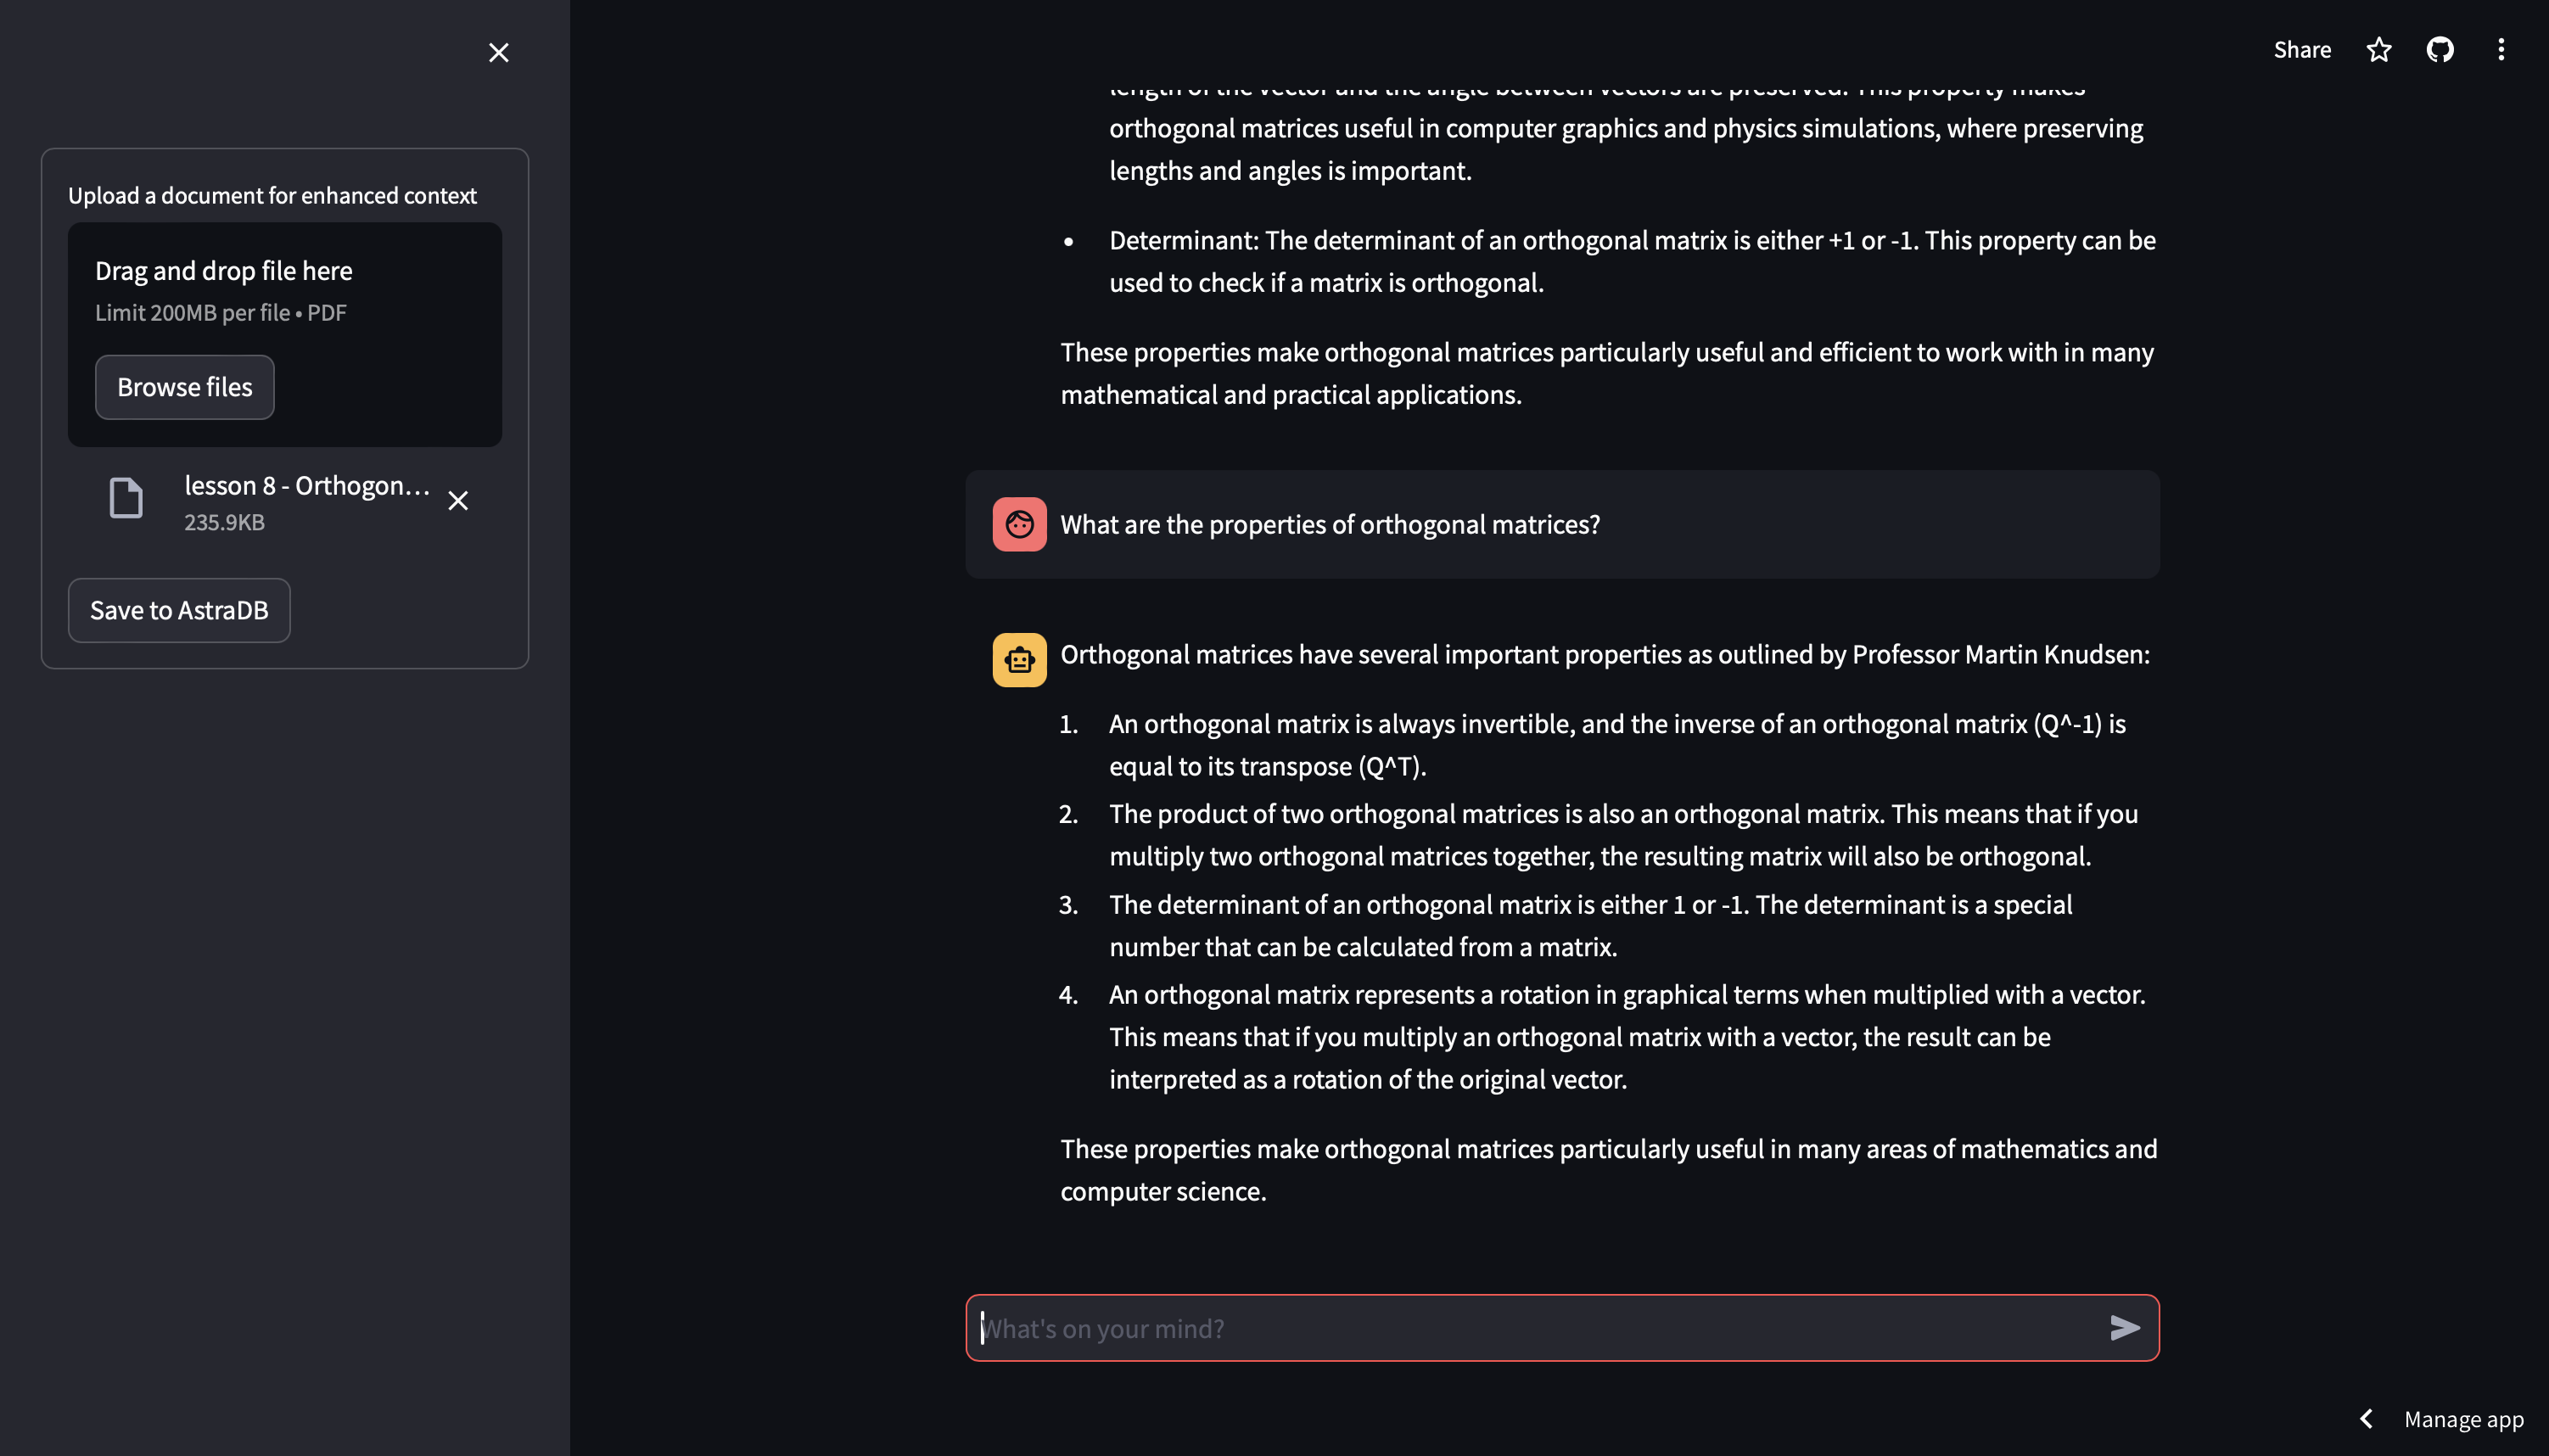
\includegraphics[width=0.8\textwidth]{figs/AfterOrthogonal.png}
        \caption{Response after insertion of lecture slides on orthogonal matrices}
        \label{fig:after_orthogonal_matrices}
    \end{figure}
    In this case we see that the professor who created the slides was referenced in the response, which was not present in the response before the document insertion. Furthermore, the response is almost identical in both structure and wording to one of the slides in the uploaded document.
\end{itemize}

\textbf{Example Query 2:}
The second query was related to an uncommon topic, e.g. a project I did earlier in my studies, and involved asking the chatbot to explain the purpose of the system developed during the project. This query was chosen to test the chatbot's ability to provide information on topics that OpenAI's GPT-4 model is not familiar with.
\begin{itemize}
    \item \textbf{Before Document Insertion:} A response was produced but lacked detailed information and context about the project. 
    \begin{figure}[H]
        \centering
        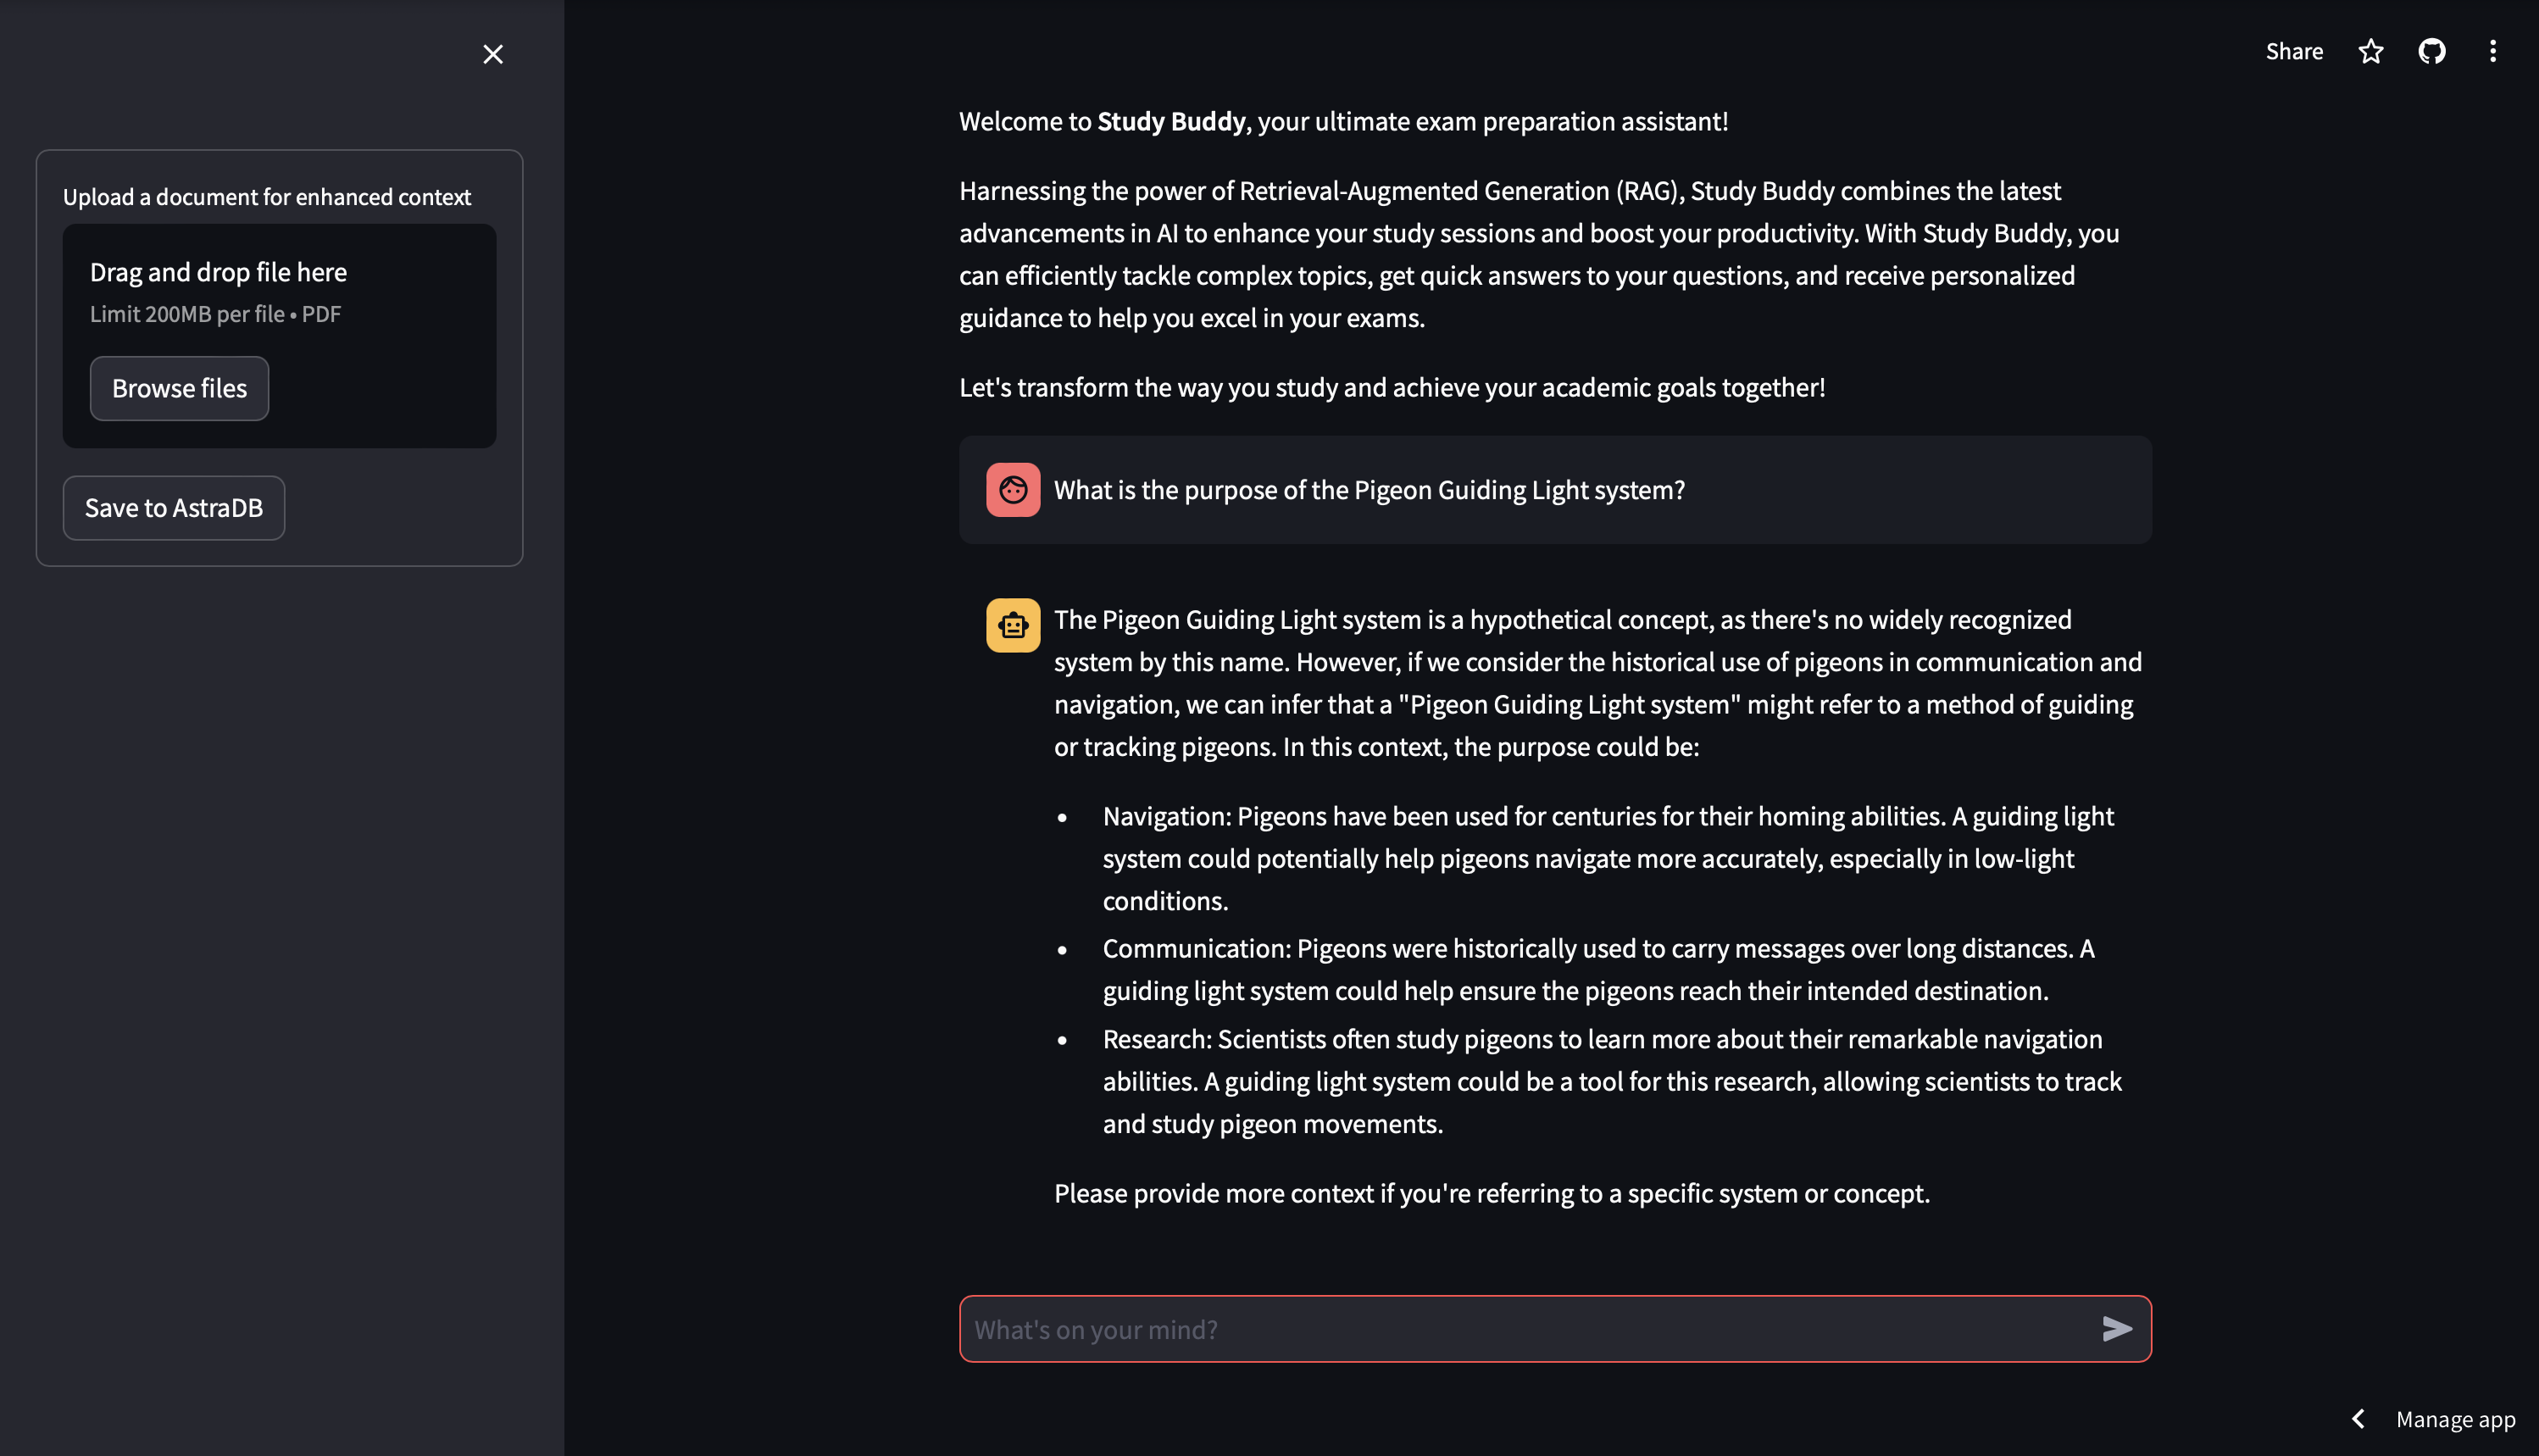
\includegraphics[width=0.8\textwidth]{figs/BeforePGL.png}
        \caption{Response before insertion of project documentation}
        \label{fig:before_project}
    \end{figure}
    \item \textbf{After Document Insertion:} The response included a detailed explanation in bullet points of the project, providing fast insight to a project that is not accesible for ChatGPT-4.
    \begin{figure}[H]
        \centering
        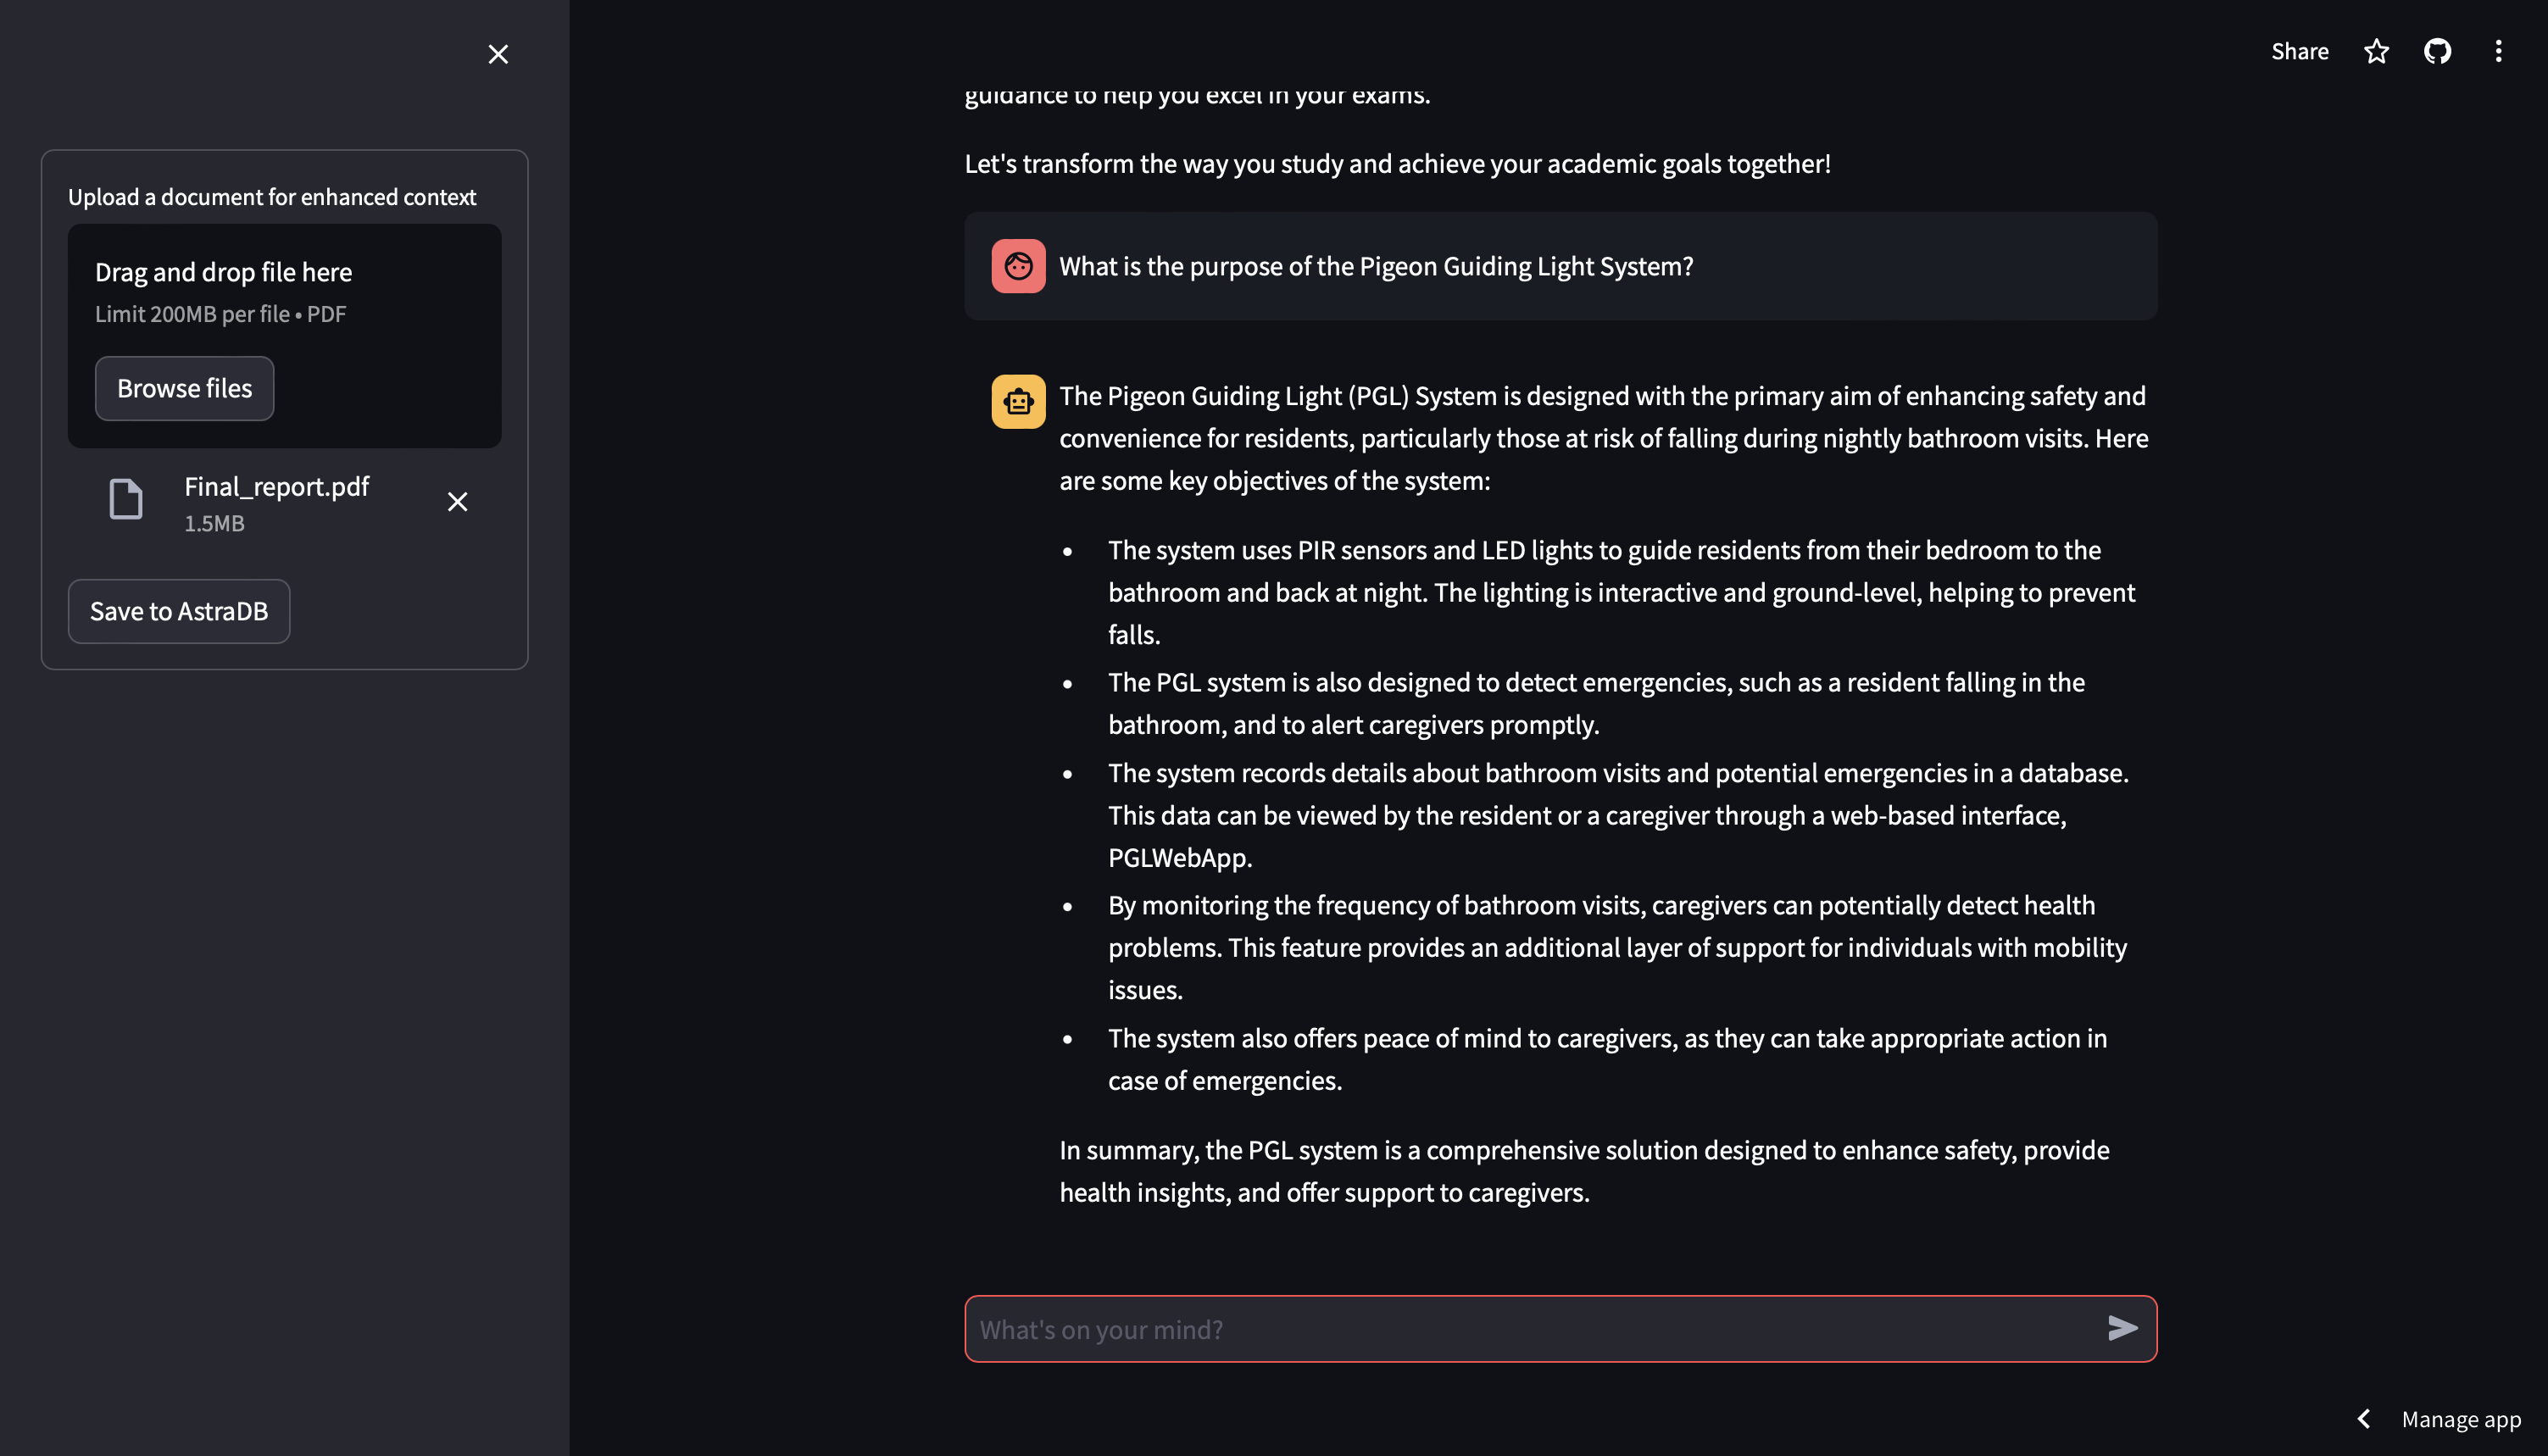
\includegraphics[width=0.8\textwidth]{figs/AfterPGL.png}
        \caption{Response after insertion of project documentation}
        \label{fig:after_project}
    \end{figure}
\end{itemize}

\subsection{Impact of Document Insertion on Unrelated Query Response}
\begin{itemize}
    \item \textbf{Document Insertion of a Single Document:} After inserting only a document on "orthogonal matrices," a query was made on a different topic, e.g. "eigenvectors". The chatbot was not able to provide a relevant response, indicating that the document insertion did impact the chatbot's ability to respond to unrelated queries.
    \begin{figure}[H]
        \centering
        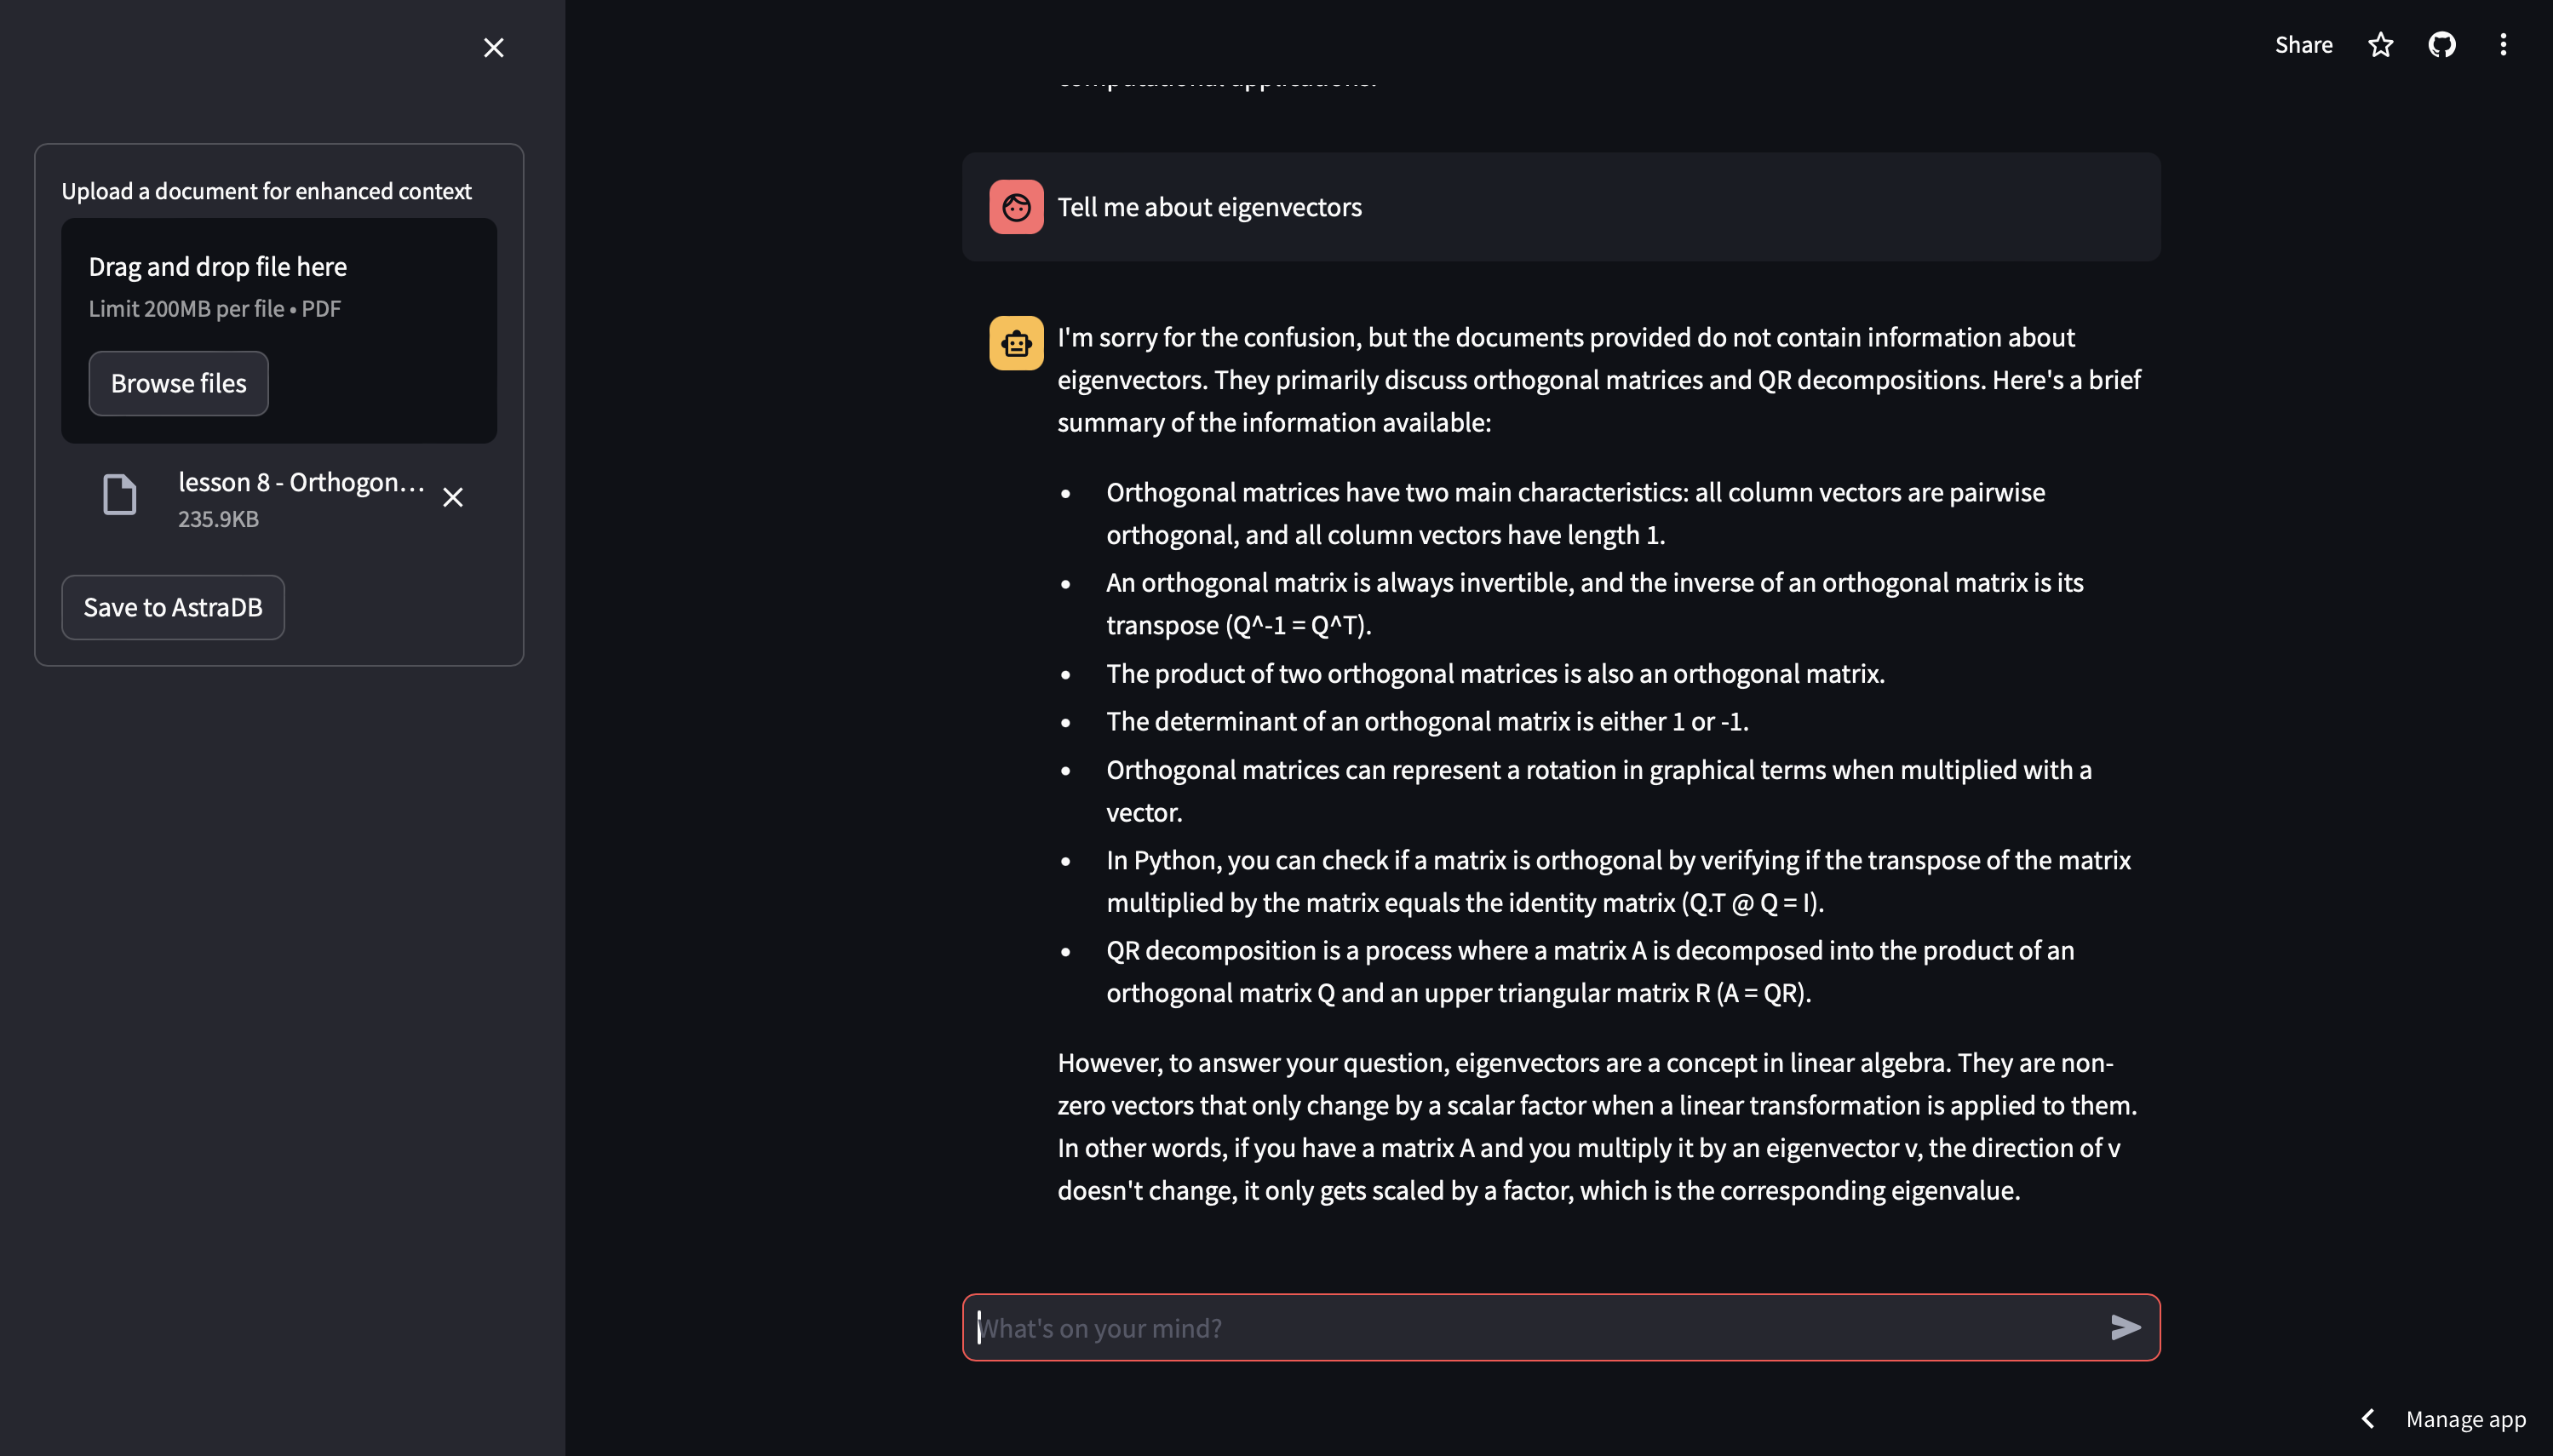
\includegraphics[width=0.8\textwidth]{figs/eigvectors.png}
        \caption{Response to an unrelated query after insertion of orthogonal matrices slides}
        \label{fig:unrelated_query}
    \end{figure}

    \item \textbf{Document Insertion of Multiple Documents:} After inserting another document on "eigenvectors," the chatbot was able to provide a relevant response to the same query on "eigenvectors." This demonstrates that the chatbot's ability to respond to queries on different topics can be improved by inserting the relevant documents.
    \begin{figure}[H]
        \centering
        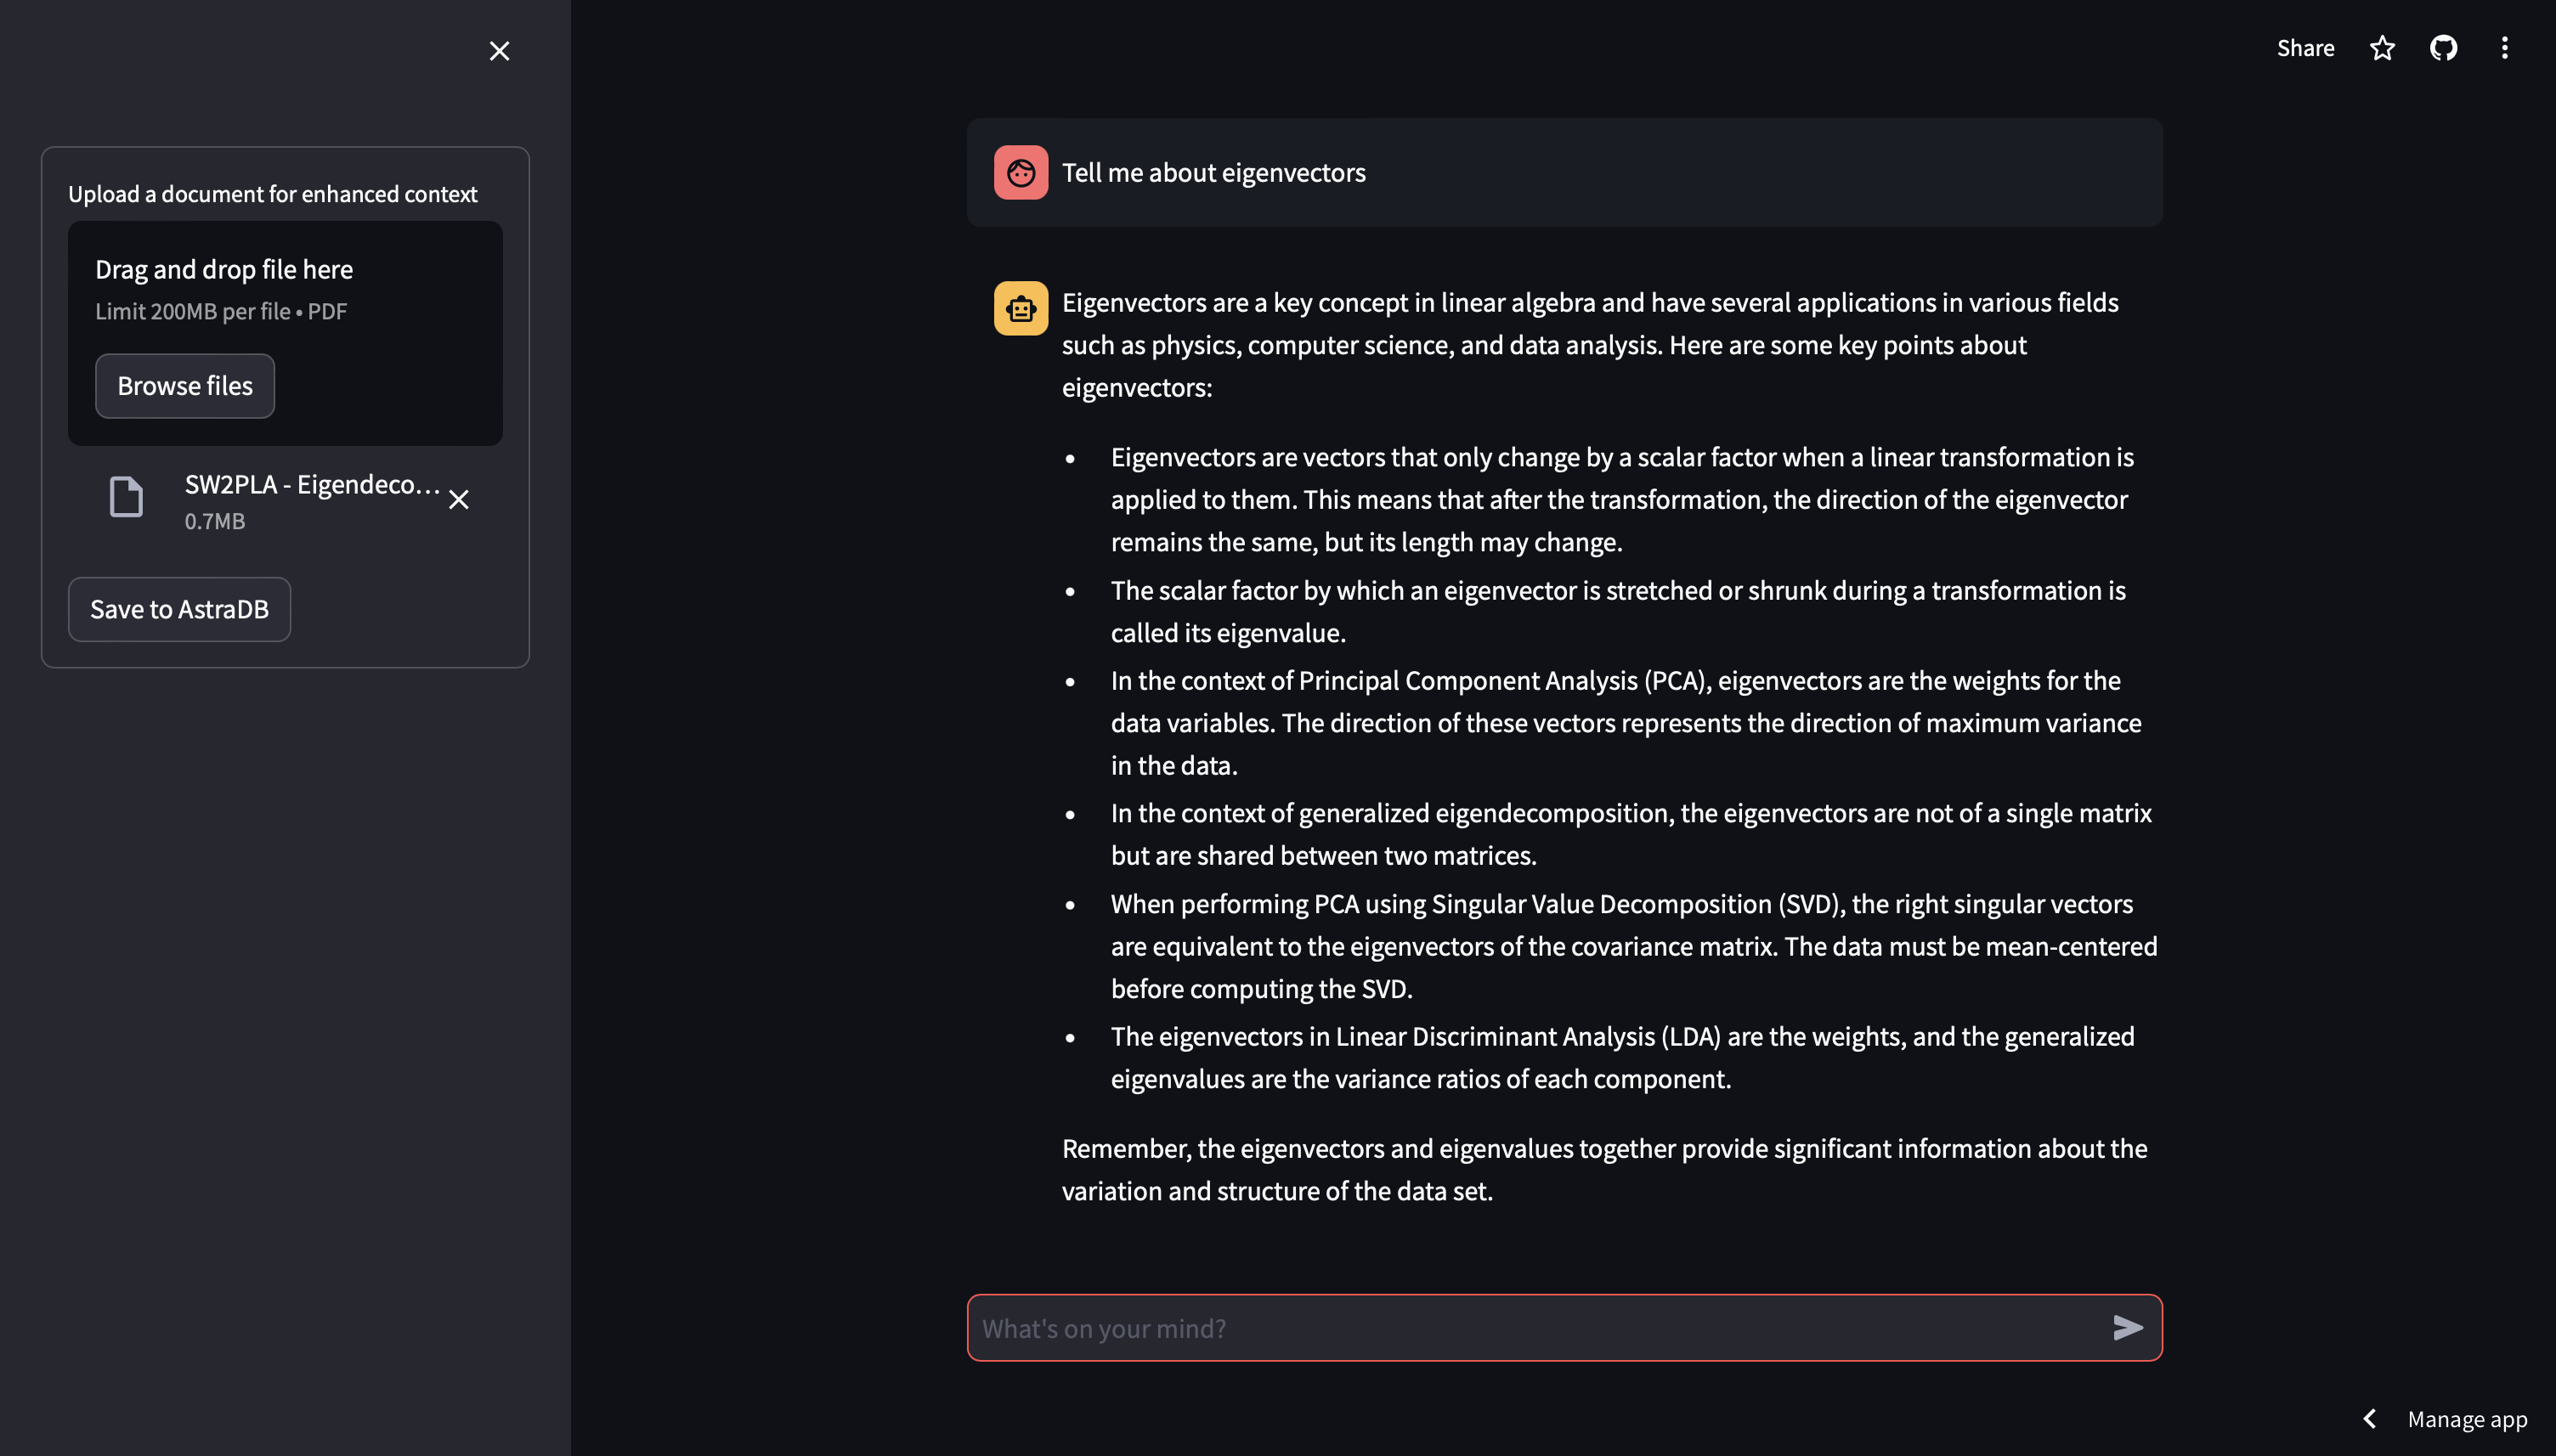
\includegraphics[width=0.8\textwidth]{figs/eigvectors2.png}
        \caption{Response to query after insertion of eigenvectors slides}
        \label{fig:unrelated_query2}
    \end{figure}
    It should be noticed that the response is tailored after the inserted document, such that it also covers PCA and SVD, which are specifically stated as related topics in the slides.
\end{itemize}
%---------------------------------------------------------------------------------------------------------------------------------------------------------------------------------------------------------------------------------------------------------------------------------

\section{Case Study}
The evaluation of compressing the BART-base and BART-large model using low-rank approximation reveals the following insights:

\subsection{ROUGE scores} The low-rank approximation technique achieves comparable ROUGE scores until rank \(r = 510\), after which the scores begin to decline. This indicates that the model's performance is preserved up to a certain rank, beyond which the approximation starts to impact the summarization quality. The following figures illustrate the ROUGE scores for various ranks:

\begin{figure}[H]
    \centering
    \begin{subfigure}[b]{0.45\textwidth}
        \centering
        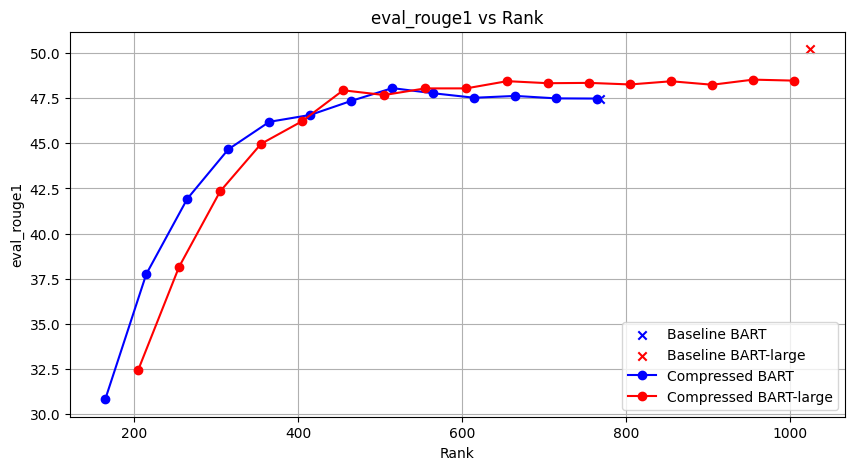
\includegraphics[width=\textwidth]{figs/06:05/Rouge1.png}
        \caption{ROUGE-1 scores.}
        \label{fig:sub1}
    \end{subfigure}
    \hfill
    \begin{subfigure}[b]{0.45\textwidth}
        \centering
        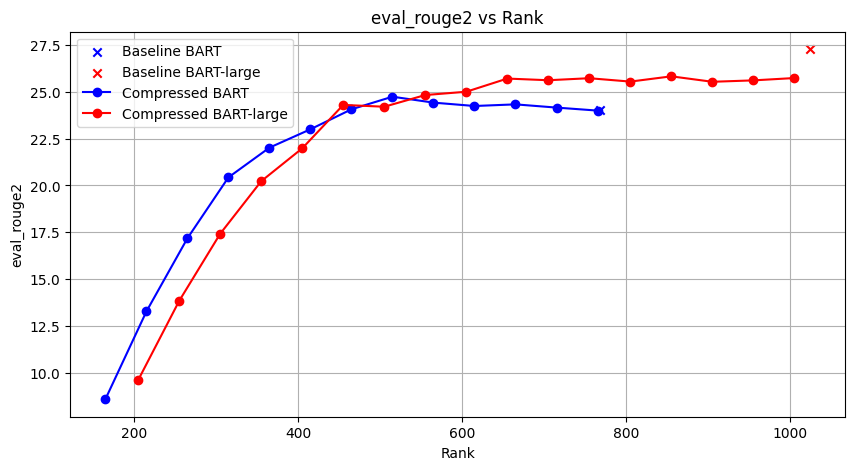
\includegraphics[width=\textwidth]{figs/06:05/Rouge2.png}
        \caption{ROUGE-2 scores.}
        \label{fig:sub2}
    \end{subfigure}
    \vskip\baselineskip
    \begin{subfigure}[b]{0.45\textwidth}
        \centering
        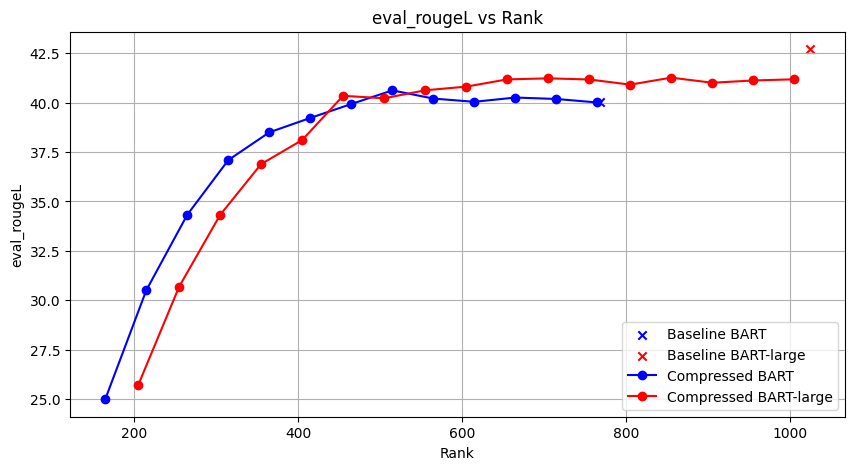
\includegraphics[width=\textwidth]{figs/06:05/RougeL.png}
        \caption{ROUGE-L scores.}
        \label{fig:sub3}
    \end{subfigure}
    \hfill
    \begin{subfigure}[b]{0.45\textwidth}
        \centering
        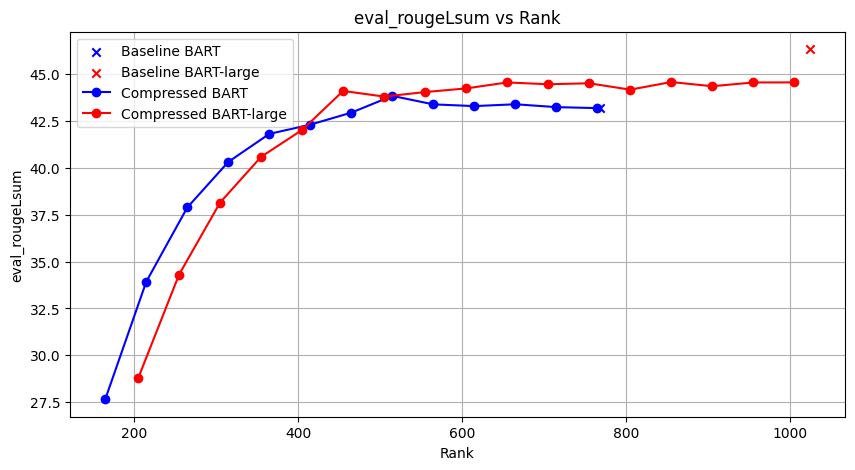
\includegraphics[width=\textwidth]{figs/06:05/RougeLSum.png}
        \caption{ROUGE-Lsum scores.}
        \label{fig:sub4}
    \end{subfigure}
    \caption{ROUGE scores for different ranks.}
    \label{fig:main}
\end{figure}

As depicted in Figure \ref{fig:main}, the ROUGE-1, ROUGE-2, ROUGE-L, and ROUGE-Lsum scores maintain a high level of performance up to a rank of \(r = 510\). However, it is important to note that for the BART-large model, there is a slight decline in performance even when the model is low-rank approximated at full rank. Beyond the rank of \(r = 510\), a noticeable degradation in scores is observed, indicating the limitations of the low-rank approximation in preserving the model's quality.

\subsection{Comparing Summaries}

The quality of the generated summaries demonstrates a noticeable decline as the rank of the low-rank approximation decreases. Initially, at higher ranks close to full rank, the summaries remain somewhat coherent and consistent, closely matching the original summary at full rank. However, as the rank decreases to \(r = 510\), the summaries start to lose details and exhibit increased errors and inconsistencies.

At ranks 765 through 730, the summary remains consistent:
\begin{quote}
    \textit{Hannah is looking for Betty's number. Amanda can't find it. Larry called her last time they were at the park together.}
\end{quote}

However, a shift is noticed at rank 725 through 720:
\begin{quote}
    \textit{Hannah doesn't know Betty's number. She texted Larry last time they were at the park together.}
\end{quote}

This slight change introduces minor variations in the narrative.

The original phrasing returns from rank 715 through 655:
\begin{quote}
    \textit{Hannah is looking for Betty's number. Amanda can't find it. Larry called her last time they were at the park together.}
\end{quote}

By rank 650 through 490, a critical detail is lost at times, but the original phrasing returns.
\begin{quote}
    \textit{Hannah is looking for Betty's number. Larry called her last time they were at the park together.}
\end{quote}

As the rank decreases further, the summary begins to diverge more substantially:
\begin{quote}
    Rank 485: \textit{Amanda can't find Betty's number. Hannah doesn't know Larry.}
\end{quote}
\begin{quote}
    Rank 470: \textit{Betty's number is not in Hannah's phone.}
\end{quote}

By the time the rank reaches around 450, the summaries are severely affected:
\begin{quote}
    Rank 435: \textit{Hannah has Betty's number. She texted Larry last time they were at the park together.}
\end{quote}

Further reduction in rank leads to highly inconsistent and erroneous summaries:
\begin{quote}
    Rank 325: \textit{Amanda can't find Betty's number. Hannah and Amanda don't know each other.}
\end{quote}
\begin{quote}
    Rank 310: \textit{Amanda and Hannah don't know each other.}
\end{quote}

At the lowest ranks, the summaries become almost nonsensical:
\begin{quote}
    Rank 205: \textit{Amanda, Hannah and Amanda are going to meet up with Larry.}
\end{quote}
\begin{quote}
    Rank 175: \textit{Amanda and Amanda don't know each other person in the park.}
\end{quote}
\begin{quote}
    Rank 150: \textit{Amanda and Amanda are going to the park.}
\end{quote}

These observations further indicates that the low-rank approximation method can maintain summarization quality up to a certain rank, beyond which the coherence and accuracy of the summaries degrade significantly. This highlights the trade-off between computational efficiency and model performance in the context of low-rank approximation.

